\section{Correcting Vignetting Effect on a PSP System}

Depending on the object, two methods for background subtraction may be performed for correcting vignetting effect. These techniques may be applied depending upon the range of height variation of a test object. 

\subsection{Direct Background Subtraction}

For plane/flat surfaces with minimal details of relative uniform depth, we used the resulting phase map itself to serve as the background. 
We took the mean of its subblocks (width x height = m x n pixels) of the image and applied bicubic interpolation.

Bicubic interpolation is a simple extension of cubic interpolation in a 2D grid \cite{Keys1981}. 
In image processing, resampling is usually done for several purposes but ultimately for refining of the image. It involves interpolation of the discrete image to a sampled continuous image \cite{Parker1983}. Bicubic interpolation is often preferred over nearest neighbor or bilinear interpolation in image resampling since it provides the smoothest interpolated surface \cite{Keys1981}. 

Figure \ref{fig:interp} shows an example of the same image interpolated using the three techniques. 
Among the three images, we see that the image interpolated using bicubic interpolation has the smoothest surface. 
Thus, we also chose bicubic interpolation to use in our method over the other two.

\begin{figure}[h!]
	\centering
	\subfigure[nearest]{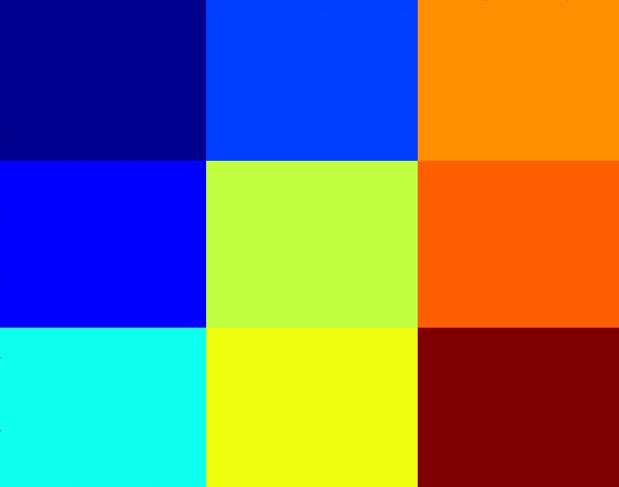
\includegraphics[height=0.25\textwidth]{figures/nearest.jpg}\label{fig:nearest}}
	\subfigure[bilinear]{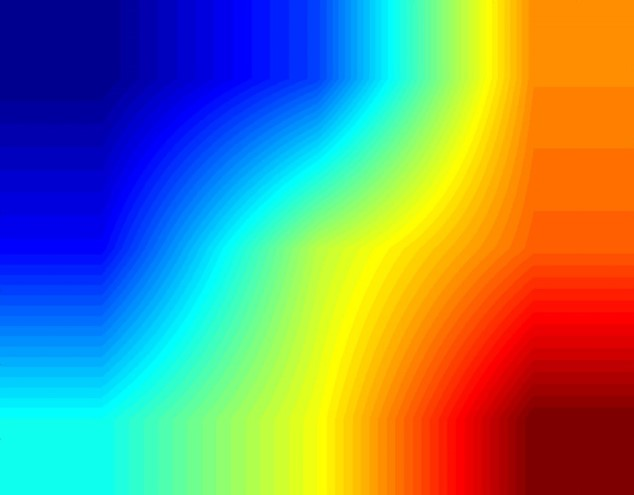
\includegraphics[height=0.25\textwidth]{figures/bilinear.jpg}\label{fig:bilinear}}
	\subfigure[bicubic]{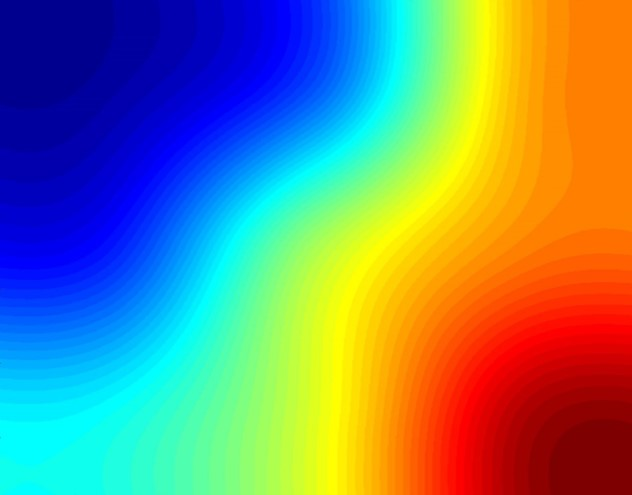
\includegraphics[height=0.25\textwidth]{figures/bicubic.jpg}\label{fig:bicubic}}
	\caption[Different types of interpolation]{A resampled image using (a) nearest, (b) bilinear, and (c) bicubic interpolation. Bicubic interpolation provides the smoothest interpolated image.}
	\label{fig:interp}
\end{figure}

The block size was carefully chosen so as not to remove the details.
The interpolated image is then subtracted to the unprocessed phase map. We refer to this process as the Direct Background Subtraction (DBS) method.

\subsection{Reference Background Subtraction}

A different approach was used for objects of nonuniform depth/height. 
DBS may only be used for this type if phase unwrapping is done per region, i.e. nonuniform illumination is less apparent if not observable for a subregion of an image; hence, it will be easier to correct it without deforming the details (modified DBS).

However, this is a tedious and highly time consuming process especially for large images and thus, we disregarded this method. As a resolution, a white image (unto which PSP is also performed) was used as the reference and its unwrapped phase was subsequently subtracted to that of the object's unwrapped phase. We call this the Reference Background Subtraction (RBS) method.

\section{Phase Maps After Background Subtraction} 
Figure \ref{fig:stone} shows the reference's and object's unwrapped phase maps for the pebbled wall. 
We see a nonuniform phase for the reference's unwrapped phase map even if it is supposed to be a flat white image.

\captionsetup[figure]{width=5.5in}
\begin{figure}[h!]
	\centering
	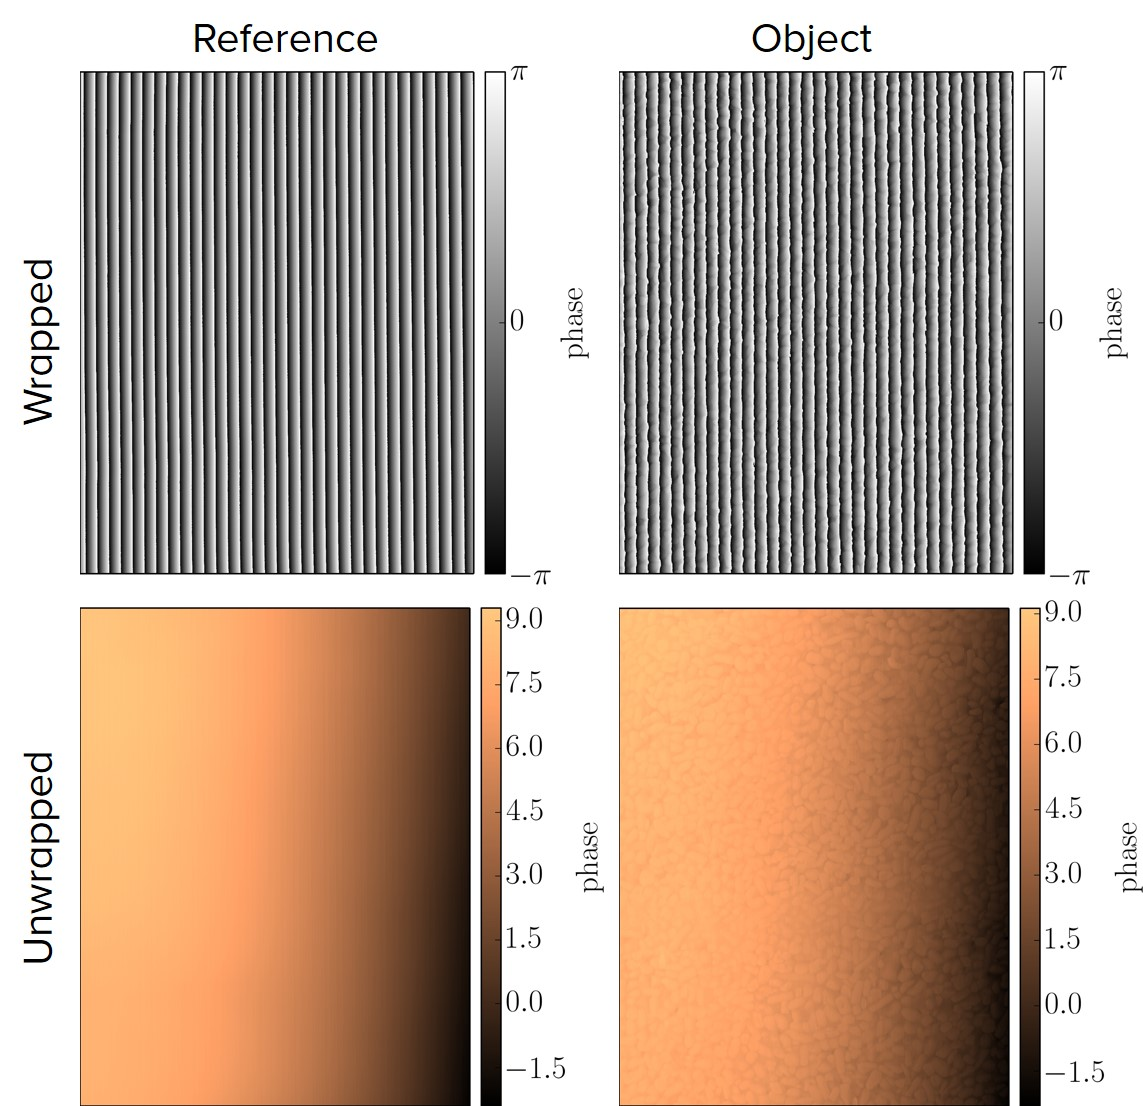
\includegraphics[width=0.765\textwidth]{figures/pebble.jpg}
	\caption[Wrapped and unwrapped phase maps of the reference and the pebbled wall]{Wrapped phase maps (top) and unwrapped phase maps (bottom) of the reference (left) and the pebbled wall (right). The images are displayed in `copper' colormap to match color of the actual object.}
	\label{fig:stone}
\end{figure}

\captionsetup[figure]{width=5in}
\begin{figure}[h!t]
	\centering
	\subfigure[RBS]{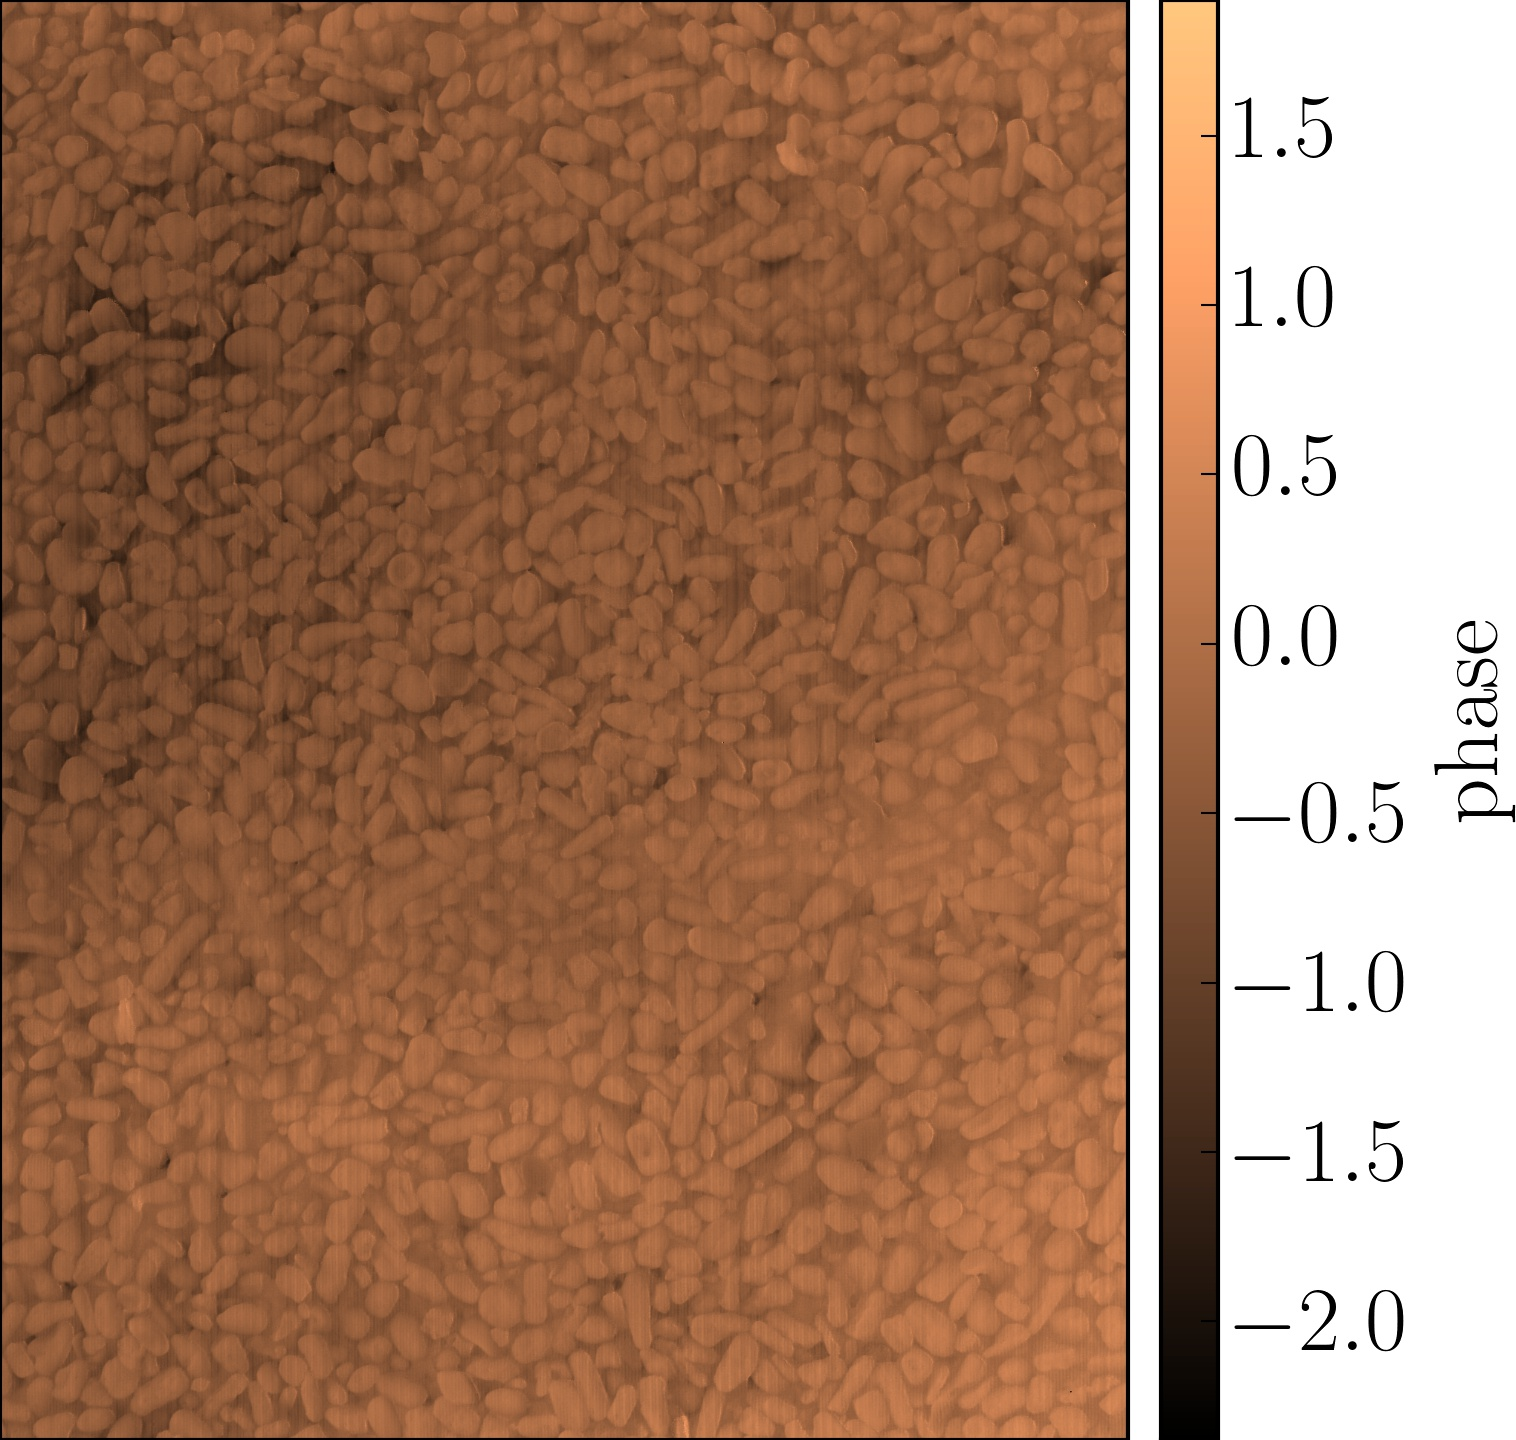
\includegraphics[width=0.42\textwidth]{figures/RBS.jpg}\label{fig:RBS}}
	\subfigure[DBS]{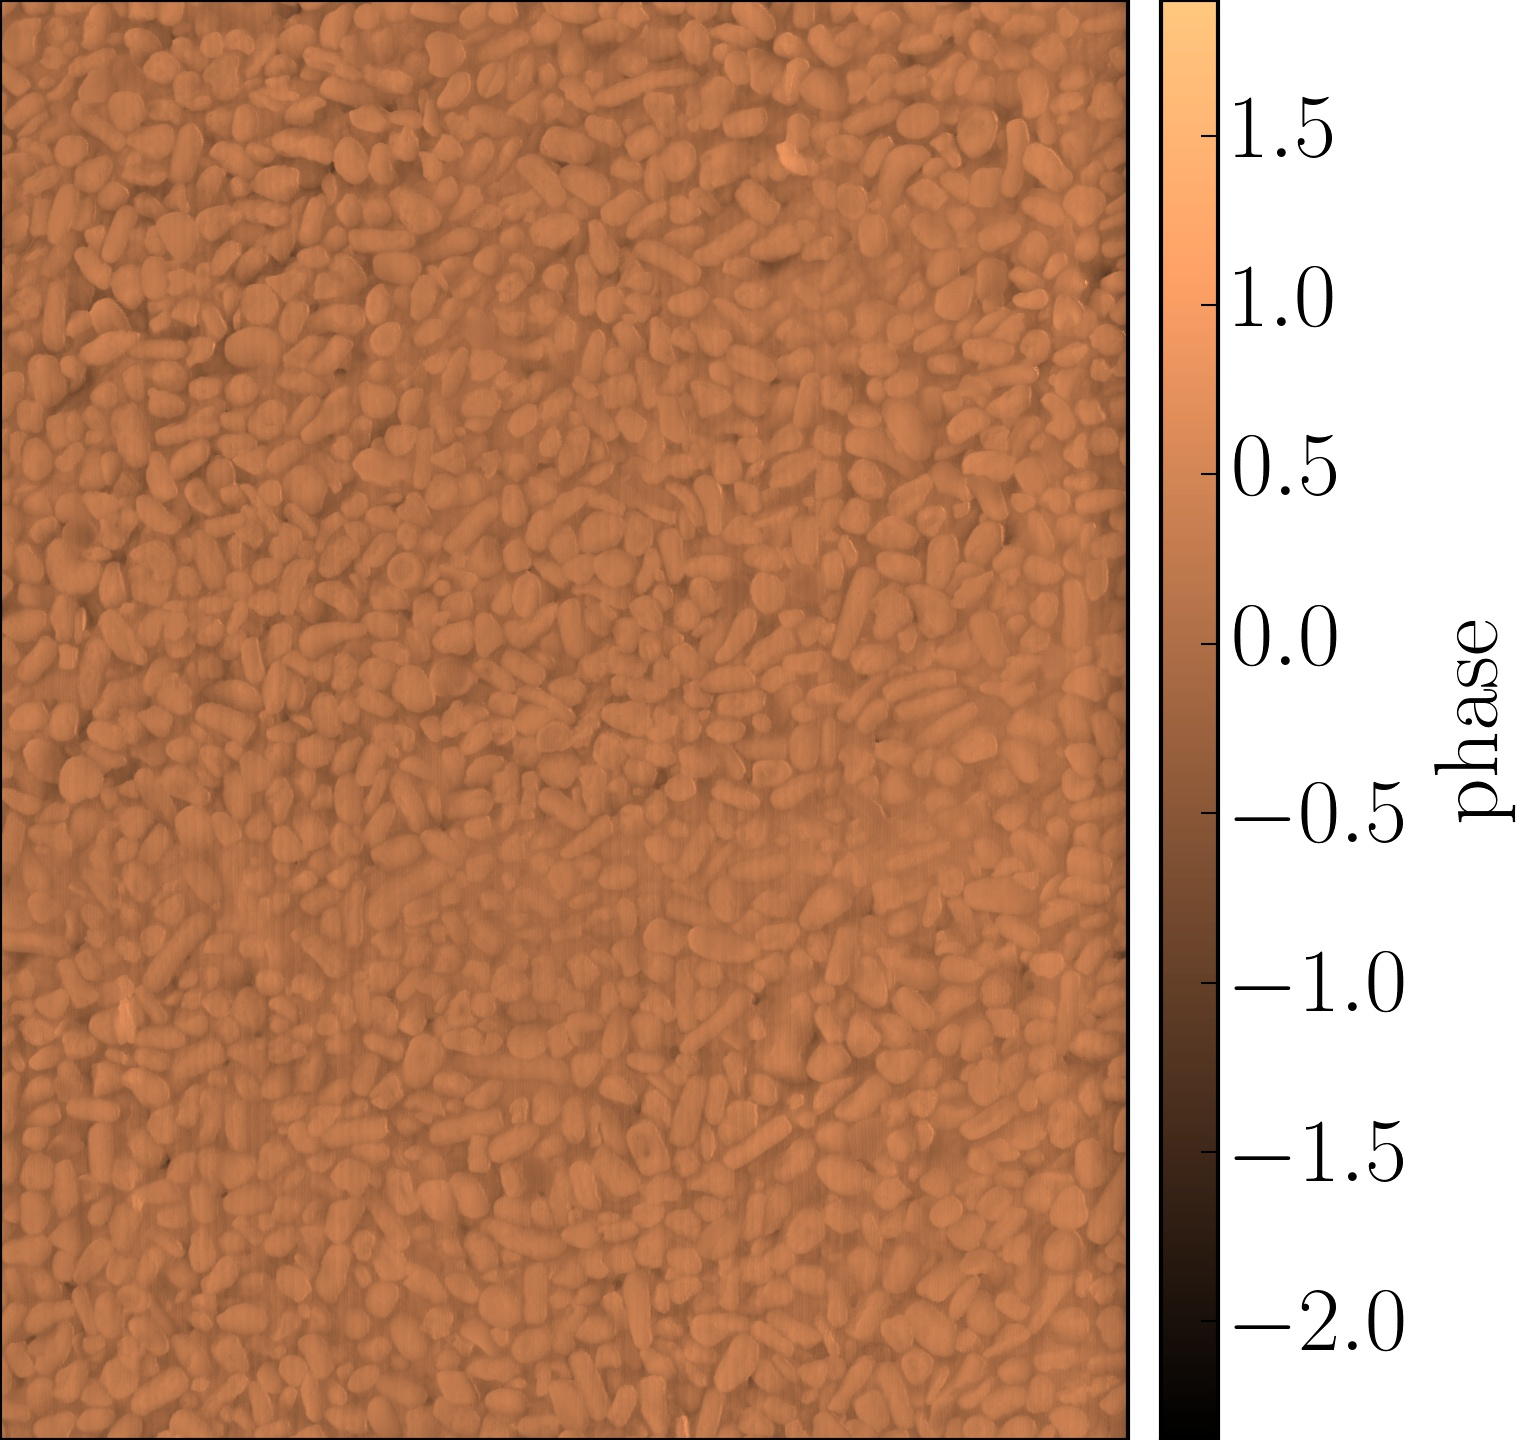
\includegraphics[width=0.42\textwidth]{figures/DBS.jpg}\label{fig:DBS}}
	\caption[Phase maps after RBS and DBS (copper colormap)]{Resulting phase maps after using (a) RBS and (b) DBS in a `copper' colormap.}
	\label{fig:stoneBS}
\end{figure}

This is an indication of the nonuniform illumination of light which is also seen in the object's unwrapped phase. 
Hence, the details of the pebbled wall are not observable.

RBS and DBS are implemented to the unwrapped phase of the pebbled wall as seen in Figure \ref{fig:stoneBS} displayed in a copper colormap with the same scale. 
The details of the pebbled wall are now observable upon application of both methods although the result of the RBS still has an apparent nonuniform intensity.

To observe this further, the phase maps were also displayed in a different colormap as shown in Figure  \ref{fig:stoneBSjet}, but still having the same scale, and we see that RBS indeed has greater contrast but is less uniform than DBS. 

\captionsetup[figure]{width=5in}
\begin{figure}[h!t]
	\centering
	\subfigure[RBS]{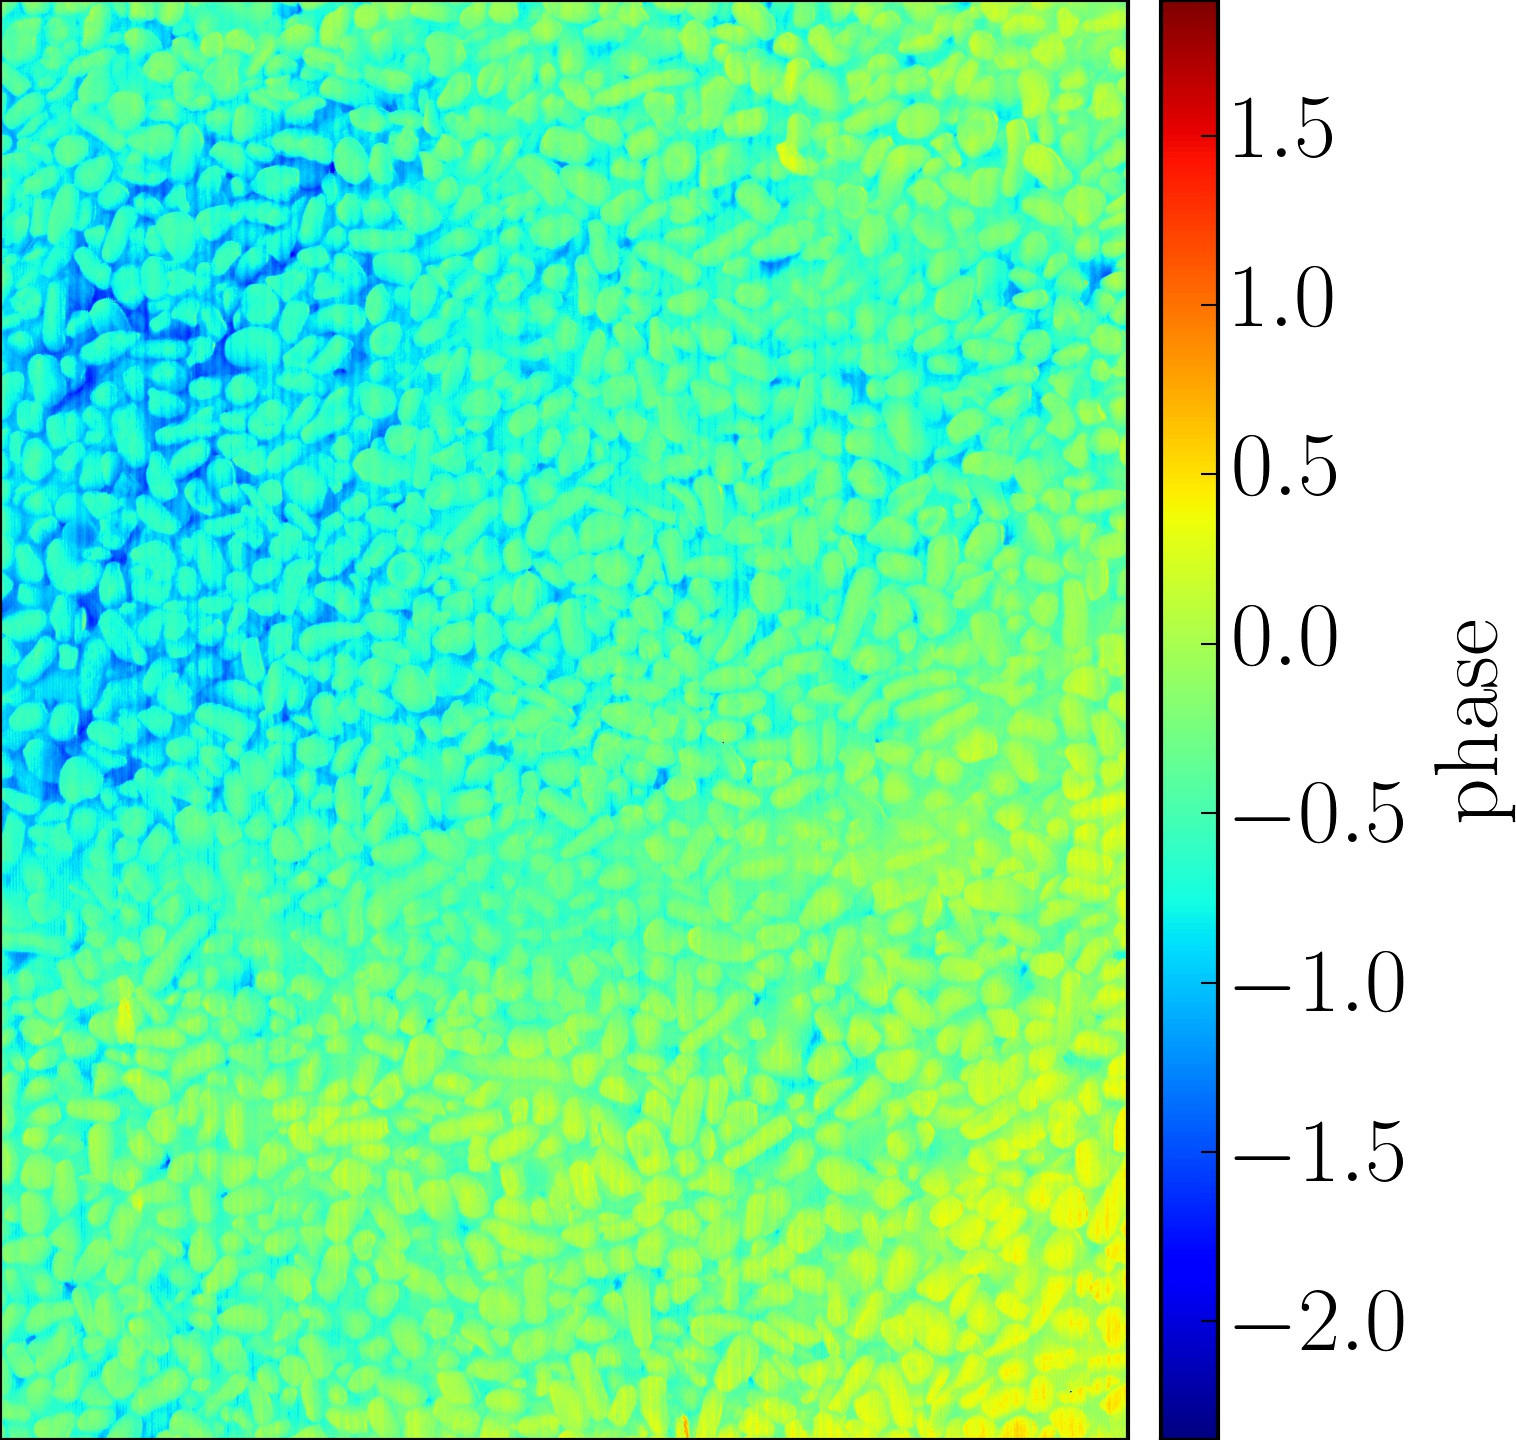
\includegraphics[width=0.42\textwidth]{figures/RBSj.jpg}\label{fig:RBS}}
	\subfigure[DBS]{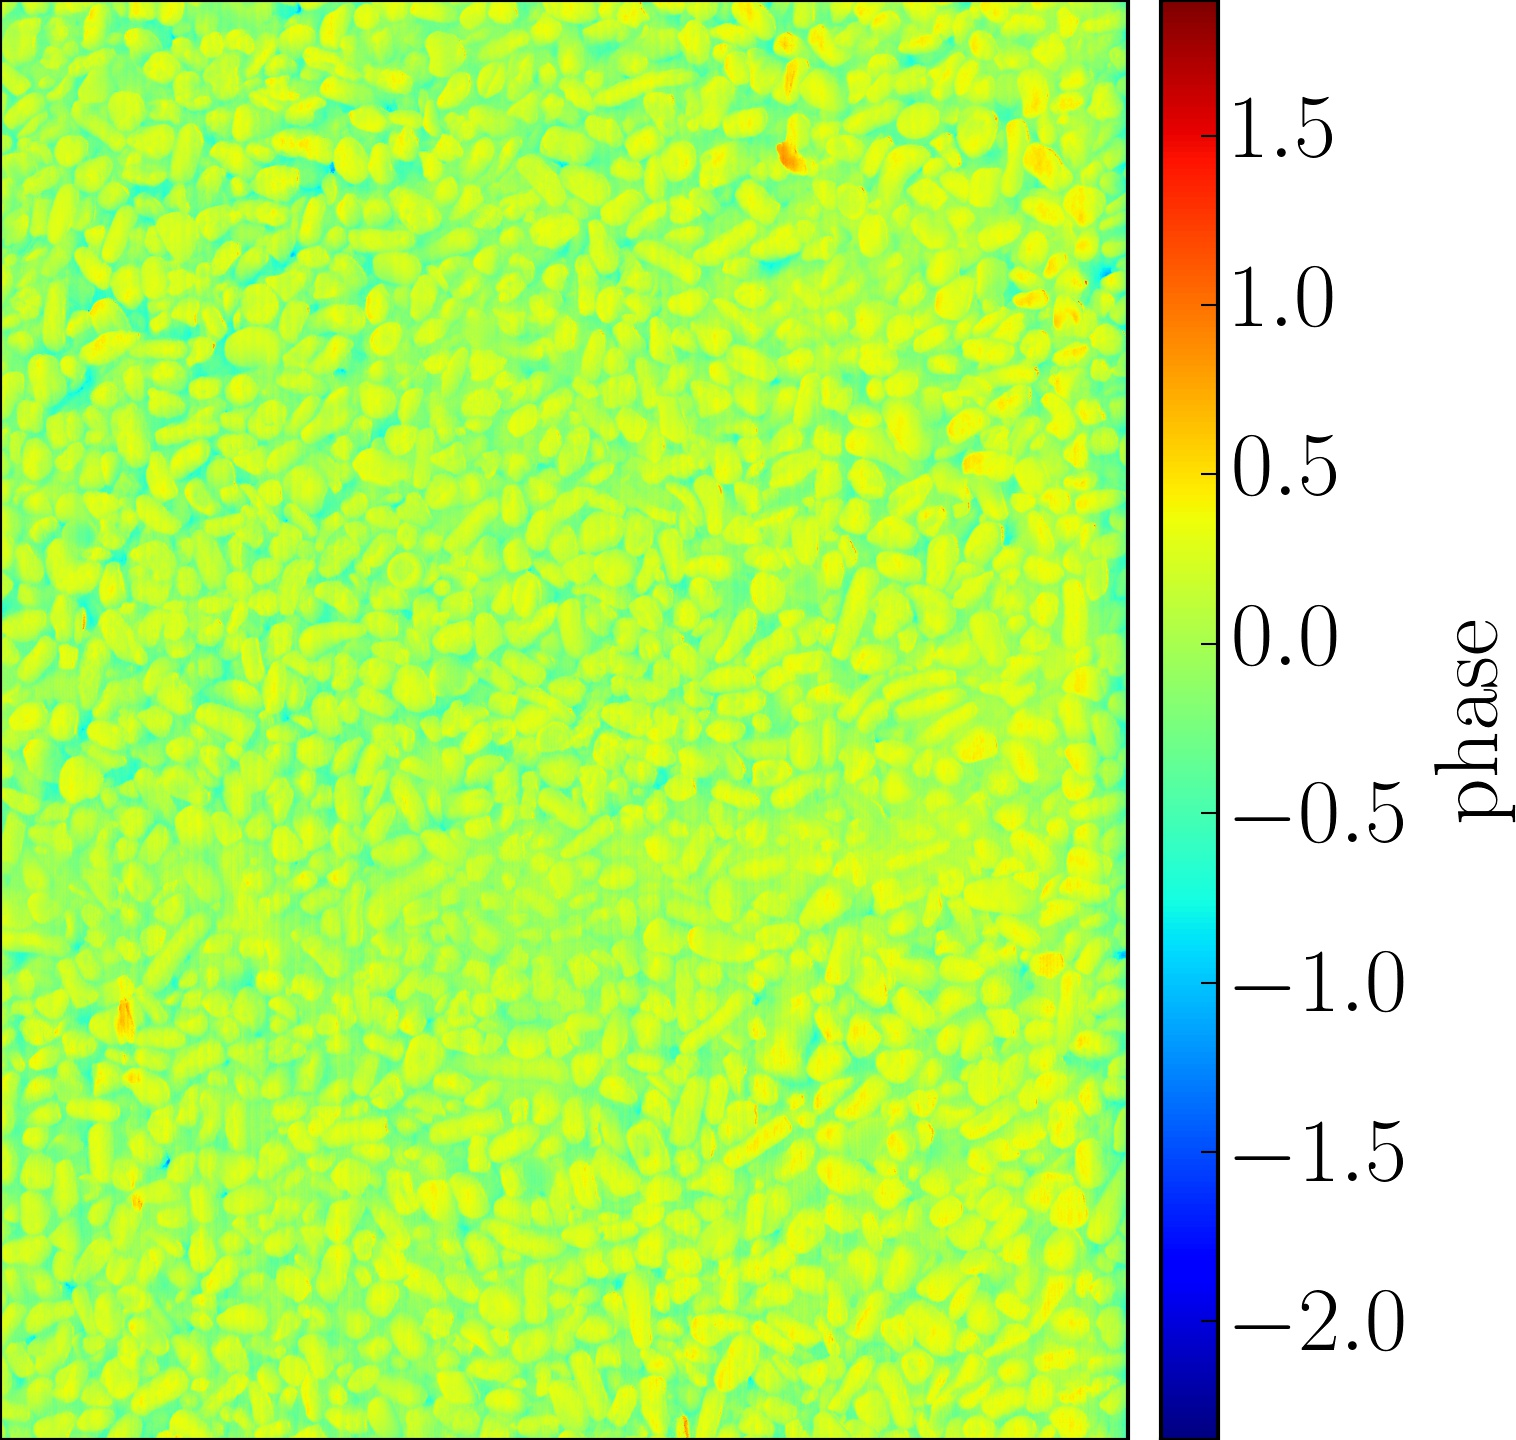
\includegraphics[width=0.42\textwidth]{figures/DBSj.jpg}\label{fig:DBS}}
	\caption[Phase maps after RBS and DBS (jet colormap)]{Resulting phase maps after using (a) RBS and (b) DBS in a `jet' colormap.}
	\label{fig:stoneBSjet}
\end{figure}

For a quantitative measurement, the histogram distributions of the phase values after application of RBS and DBS were obtained as shown in Figure \ref{fig:stonehist}. We see that the RBS has a wider distribution of phase values as compared to DBS. 

The standard deviation of the two were also obtained: RBS = 0.315, DBS = 0.201. Higher standard deviation means a higher distribution of phase values or a higher contrast. However, what we are looking at is the uniformity of the values. Thus, DBS is still has a better result.

\captionsetup[figure]{width=5in}
\begin{figure}[h!]
	\centering
	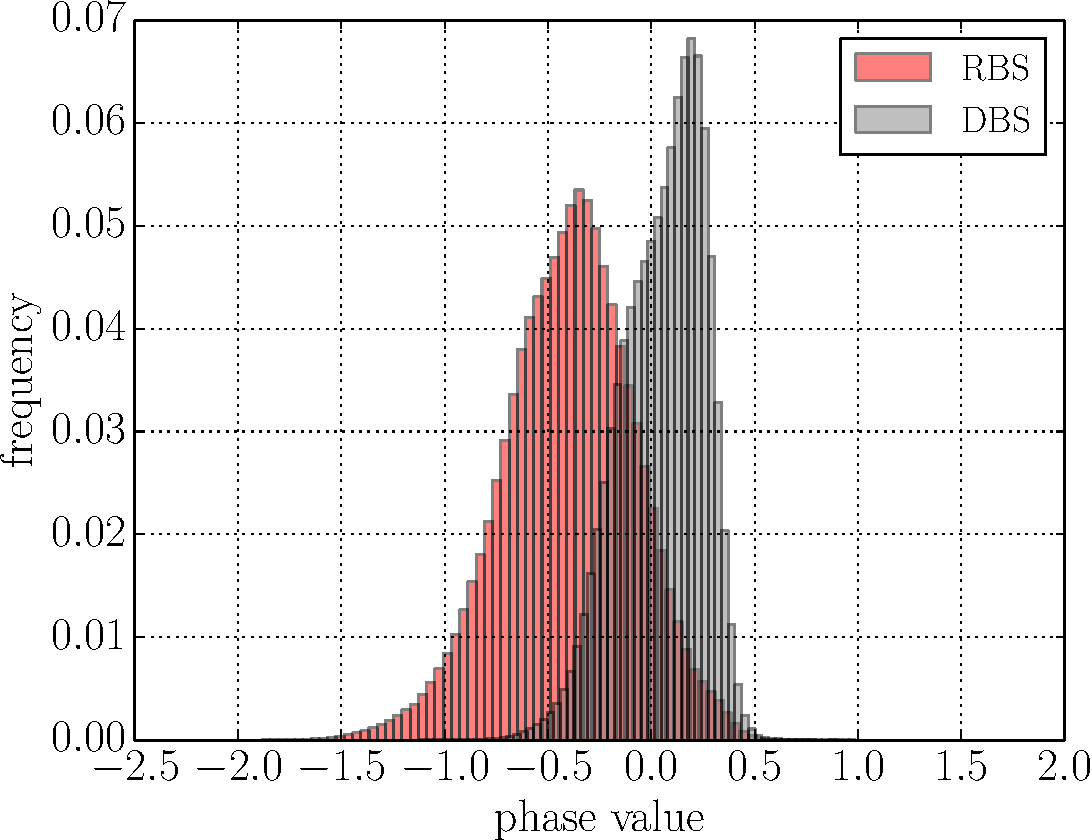
\includegraphics[width=0.62\textwidth]{figures/stonehist.pdf}
	\caption[Histogram of phase values]{Histogram distribution of phase values of the pebbled wall after RBS and DBS.}
	\label{fig:stonehist}
\end{figure}

\begin{figure}[h!]
	\centering
	\subfigure[Before DBS]{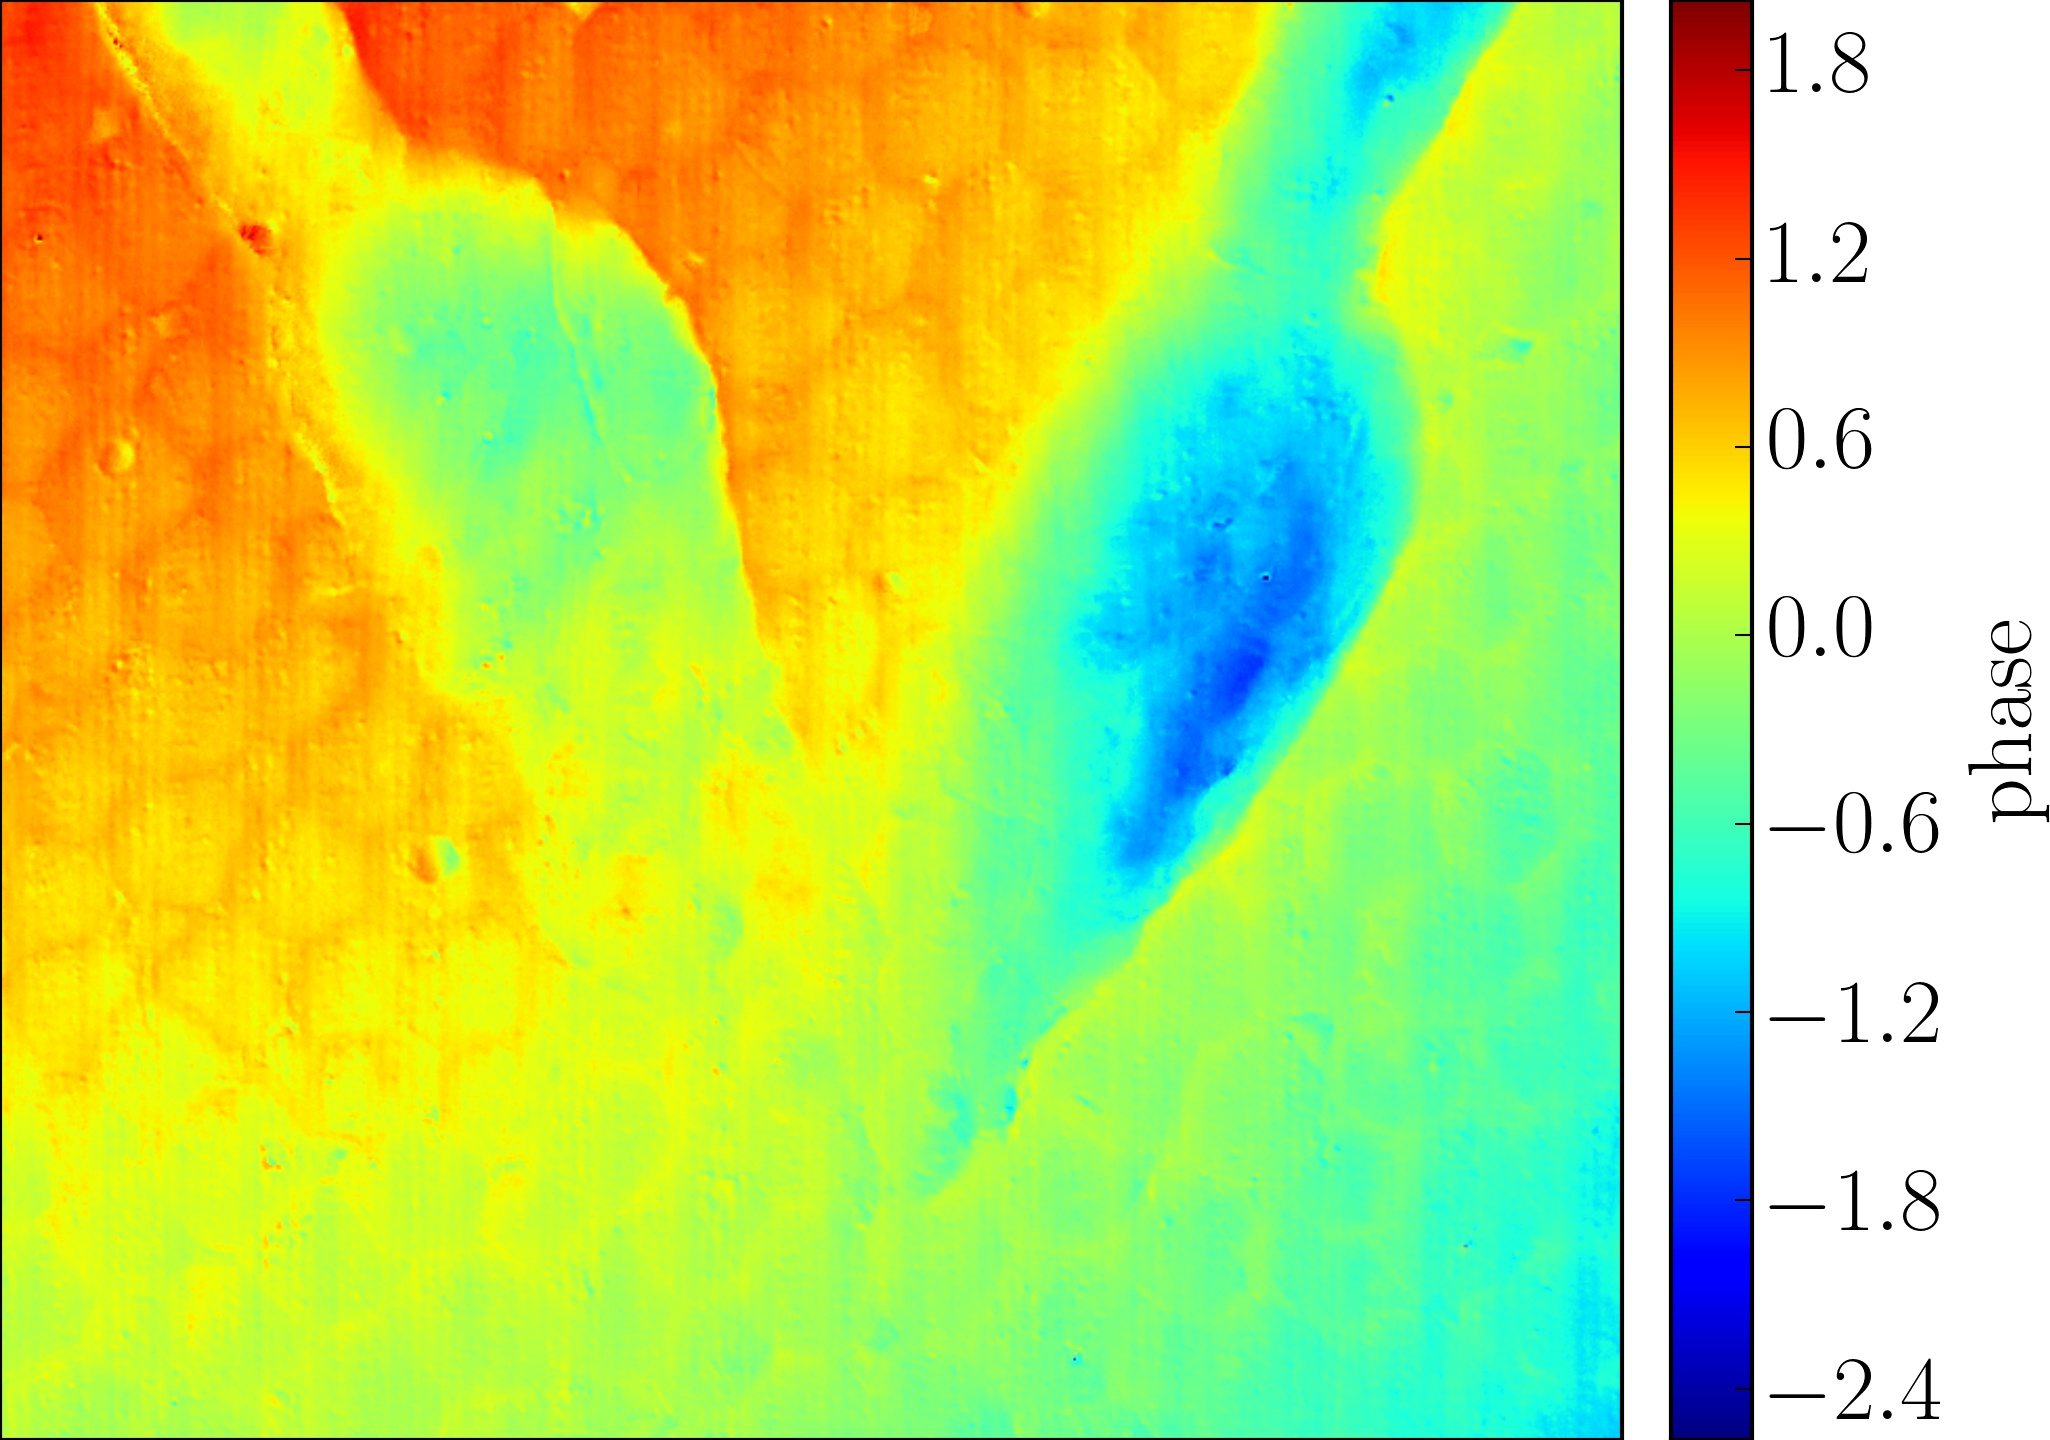
\includegraphics[width=0.42\textwidth]{figures/V.jpg}\label{fig:V}}
	\subfigure[Subtracted background]{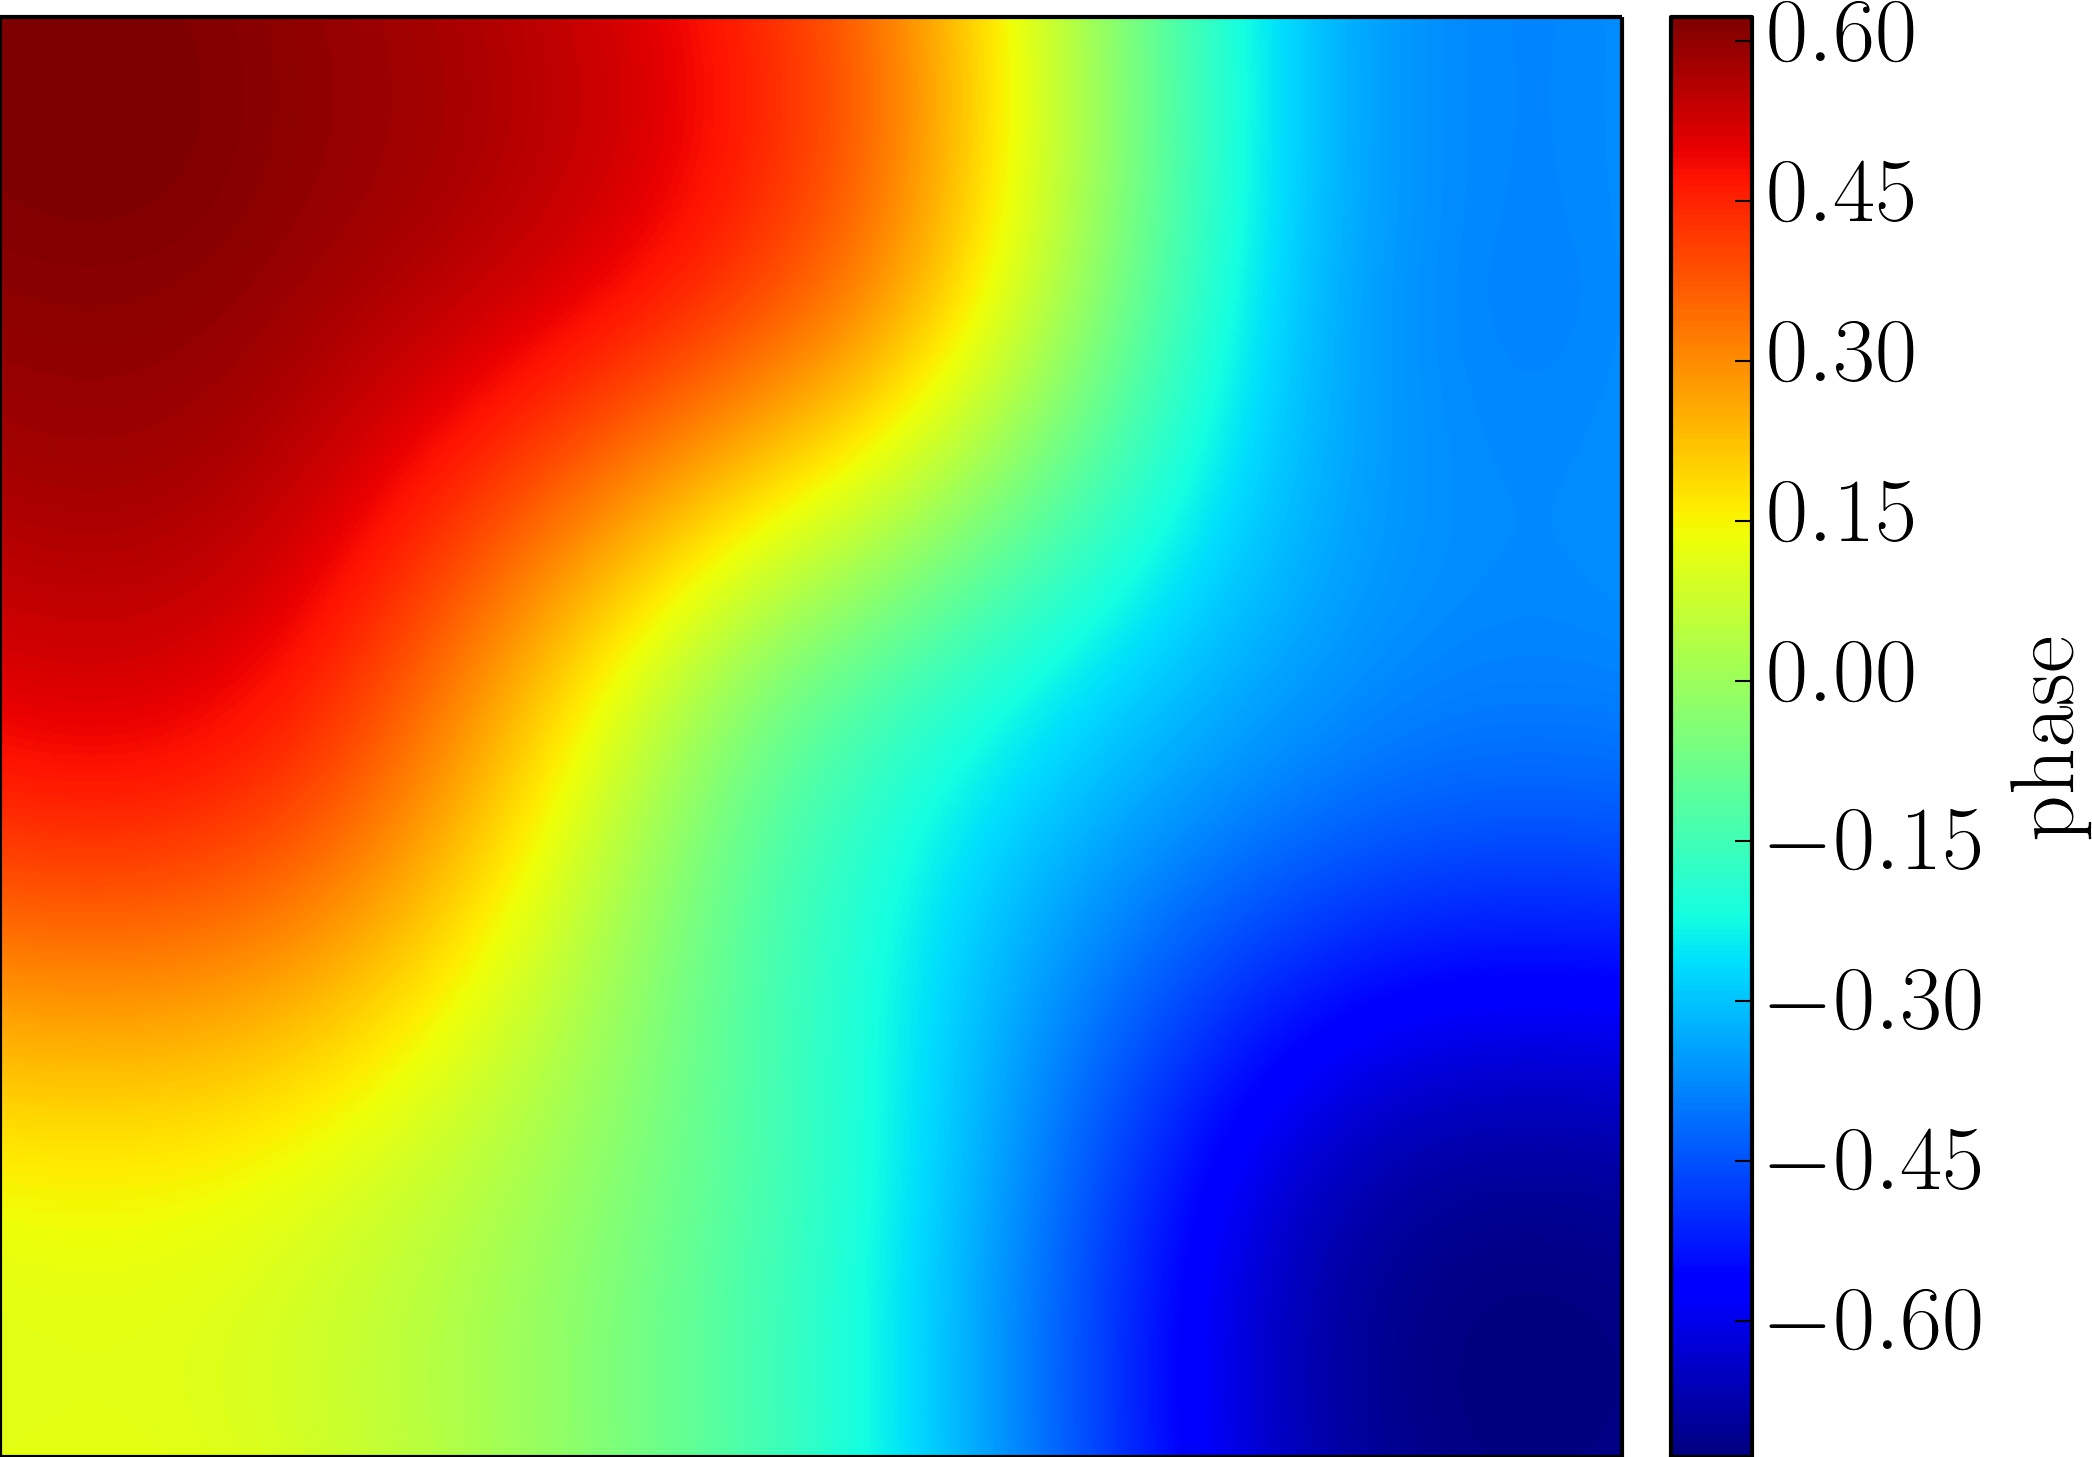
\includegraphics[width=0.42\textwidth]{figures/Vbg.jpg}\label{fig:Vbg}}
	\subfigure[After DBS]{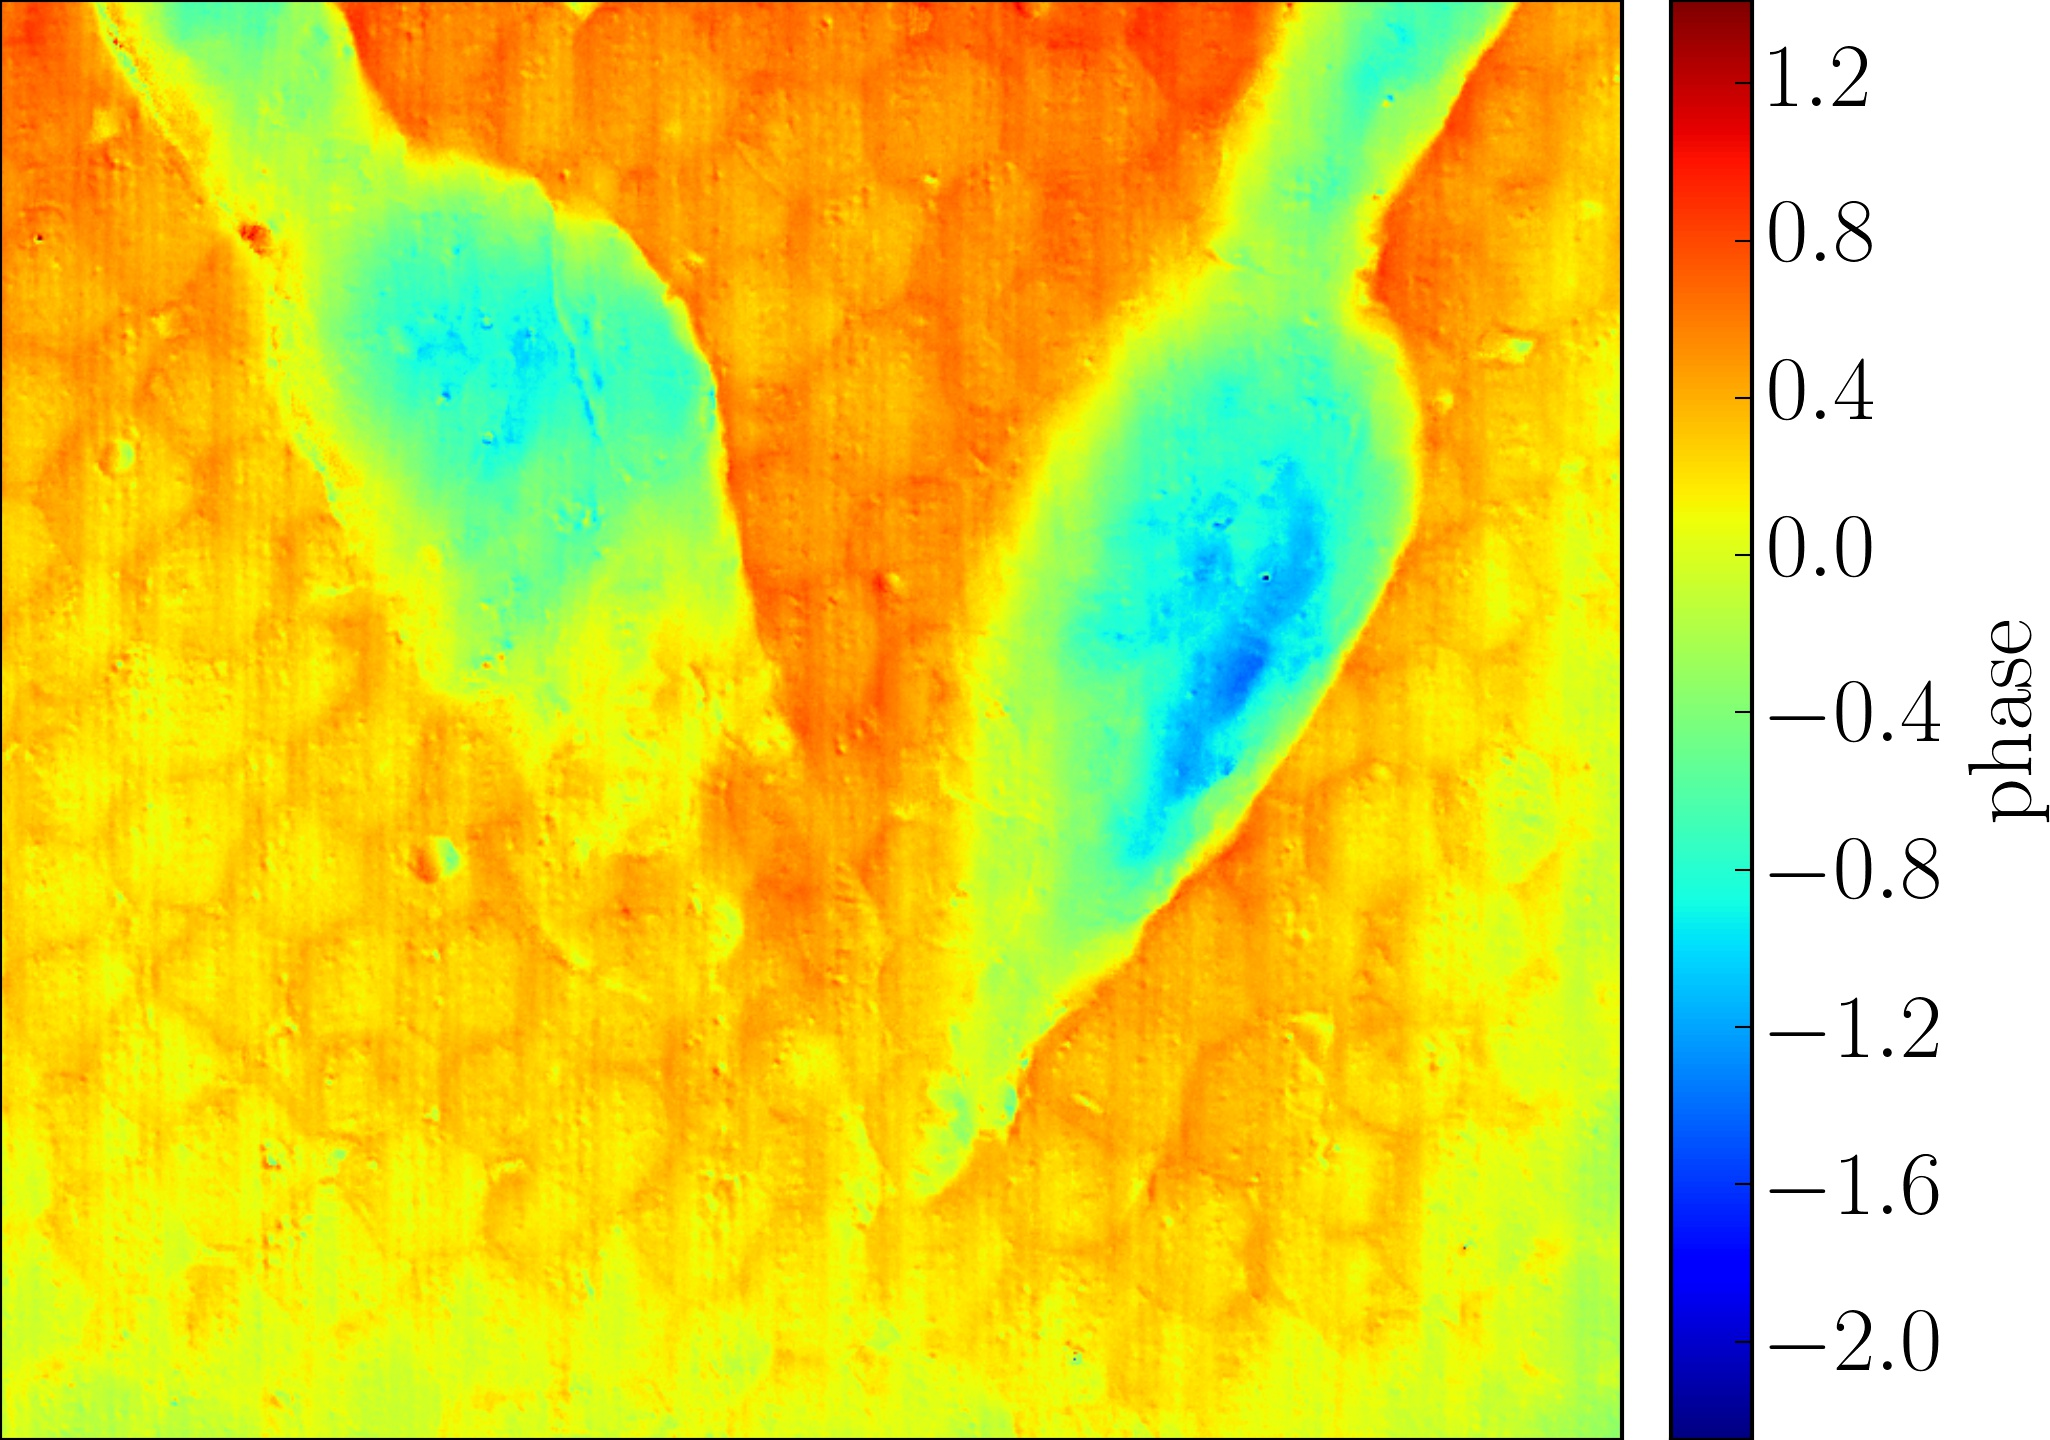
\includegraphics[width=0.42\textwidth]{figures/V_BS.jpg}\label{fig:VDBS}}
	\caption[Phase maps of styrofoam board with engravings]{Styrofoam board with engravings: (a) original phase map, (b) interpolated background, and (c) output phase map.}
	\label{fig:styroV}
\end{figure}

DBS was also applied to another relatively flat object: styrofoam board with engravings. Figure \ref{fig:styroV} shows the difference between the unprocessed phase map and the processed phase map after DBS. We notice the huge difference in the phase map before and after background subtraction.

DBS is better for flat objects with minimal details (depth/height of less than 10 mm). As for RBS, incorrectly placing the reference during the experiment will lead to discrepancies in phase values.

Figure \ref{fig:pyramid} shows the reference's and object's wrapped and unwrapped phases of a step pyramid. For the step pyramid, DBS is not applicable as taking the mean of its subblocks will give a wrong depth perception. The reference's unwrapped phase has a maximum phase value reaching approximately 0.9, while the object's unwrapped phase reaches up to approximately 9. Thus, their unwrapped phases were intendedly displayed with different scaling of phase values. 

\captionsetup[figure]{width=5in}
\begin{figure}[h!]
	\centering
	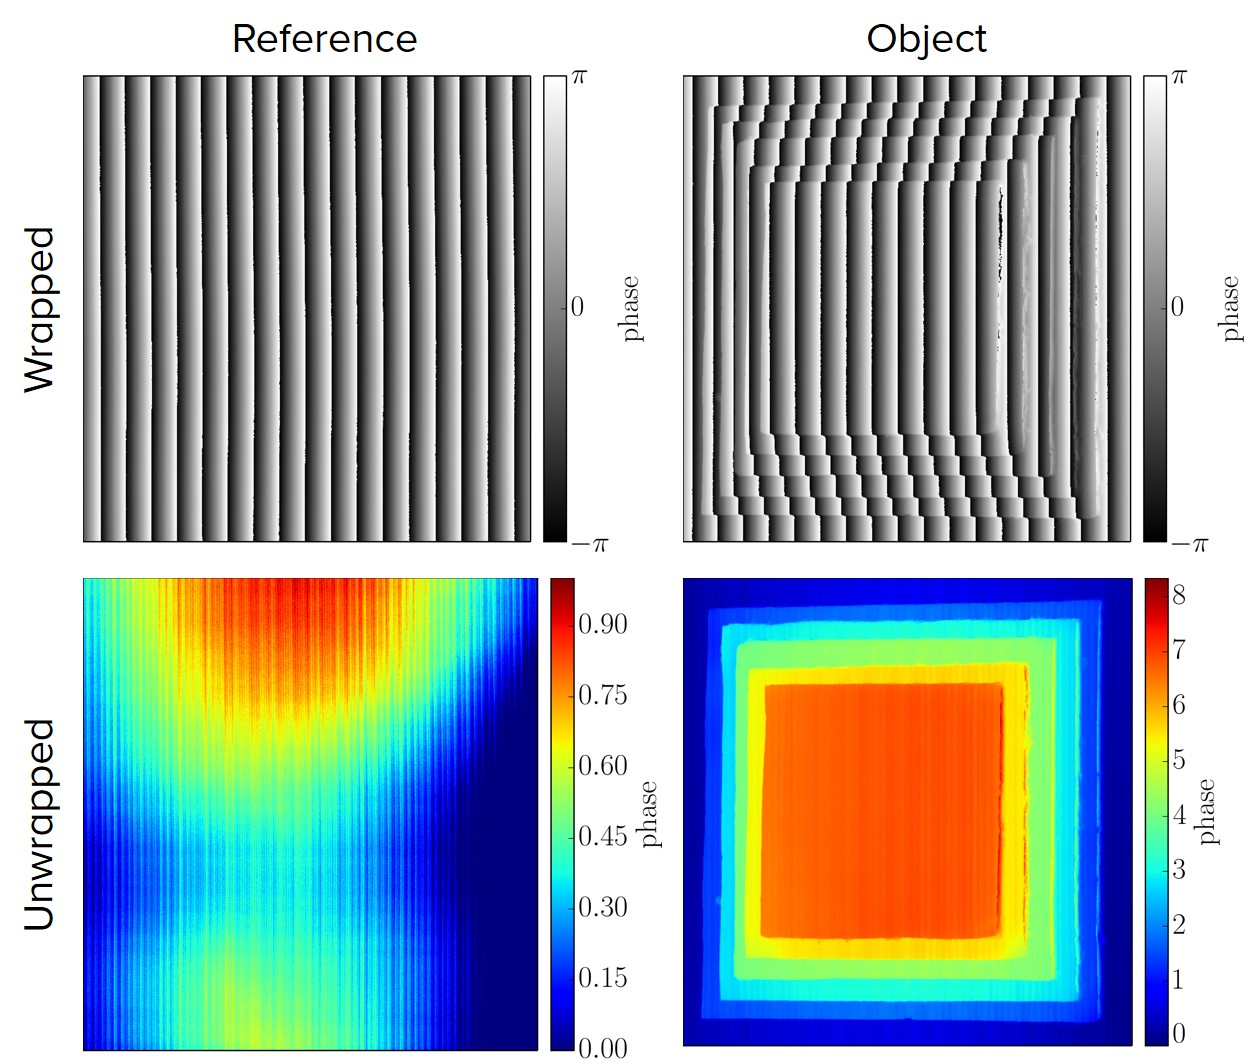
\includegraphics[width=0.75\textwidth]{figures/pyramid.jpg}
	\caption[Wrapped and unwrapped phase maps of reference and step pyramid]{Wrapped (top) and unwrapped phase maps of the reference (left) and the step pyramid (right).}
	\label{fig:pyramid}
\end{figure}

If the reference's unwrapped phase was rescaled to display the same scaling as that of the object's, we would see only a flat blue surface. It is also for this reason that subtracting the reference's unwrapped phase to the object's unwrapped phase will result to not much difference.
